\newcounter{UC}
\newcounter{SUC}
\newcounter{SSUC}

\newcommand{\resetCounter}[1]{%
    \setcounter{#1}{0}
}

\newcommand{\UseCase}[1]{%
    \refstepcounter{UC}
    \resetCounter{SUC}
    \resetCounter{SSUC}
    \subsection{UC\arabic{UC} - #1}\label{UC:\arabic{UC}}
}

\newcommand{\SubUseCase}[1]{%
    \stepcounter{SUC}
    \resetCounter{SSUC}
    \subsubsection{UC\arabic{UC}.\arabic{SUC} - #1}
}

\newcommand{\SubSubUseCase}[1]{%
    \stepcounter{SSUC}  
    \paragraph{UC\arabic{UC}.\arabic{SUC}.\arabic{SSUC} - #1}
}

% COME UTILIZZARE I CASI D`USO:
% i comandi di use case vanno utilizzati al posto di subsection, subsubsection e paragraph

% \UseCase => rappresenta lo use case principale (UC1,UC2,UC3)
% \SubUseCase => rappresenta il primo sotto livello dello use case principale (UC1.1,UC2.1,UC3.3)
% \SubSubUseCase => rappresenta il secondo sotto livello dello lo use case principale (UC1.1.1,UC2.1.2,UC3.3.1)

\newcommand{\UCdsc}[5]{
    \begin{itemize}
        \item \textbf{Attore primario:}
         #1
        \item \textbf{Descrizione:} 
         #2
        \item \textbf{Precondizioni:}
         #3
        \item \textbf{Postcondizioni:}
        #4
        \item \textbf{Scenario principale:} 
         #5
    \end{itemize}
}


\GetTitleStringSetup{expand}
\section{Casi d'uso}
% \subsection{Attore}
% Poiché per lo svolgimento del progetto non è necessario gestire permessi differenti per l'accesso alle funzionalità, l'attore che interagisce con il nostro software è unico, denominato "Utente".\\
% \textbf{Utente:} soggetto che utilizza la web application, sfruttandone le funzionalità.


% UC1 - UC11




%UC12 - UC19
\UseCase{Zoom della vista}
\begin{figure}[h!]\centering
    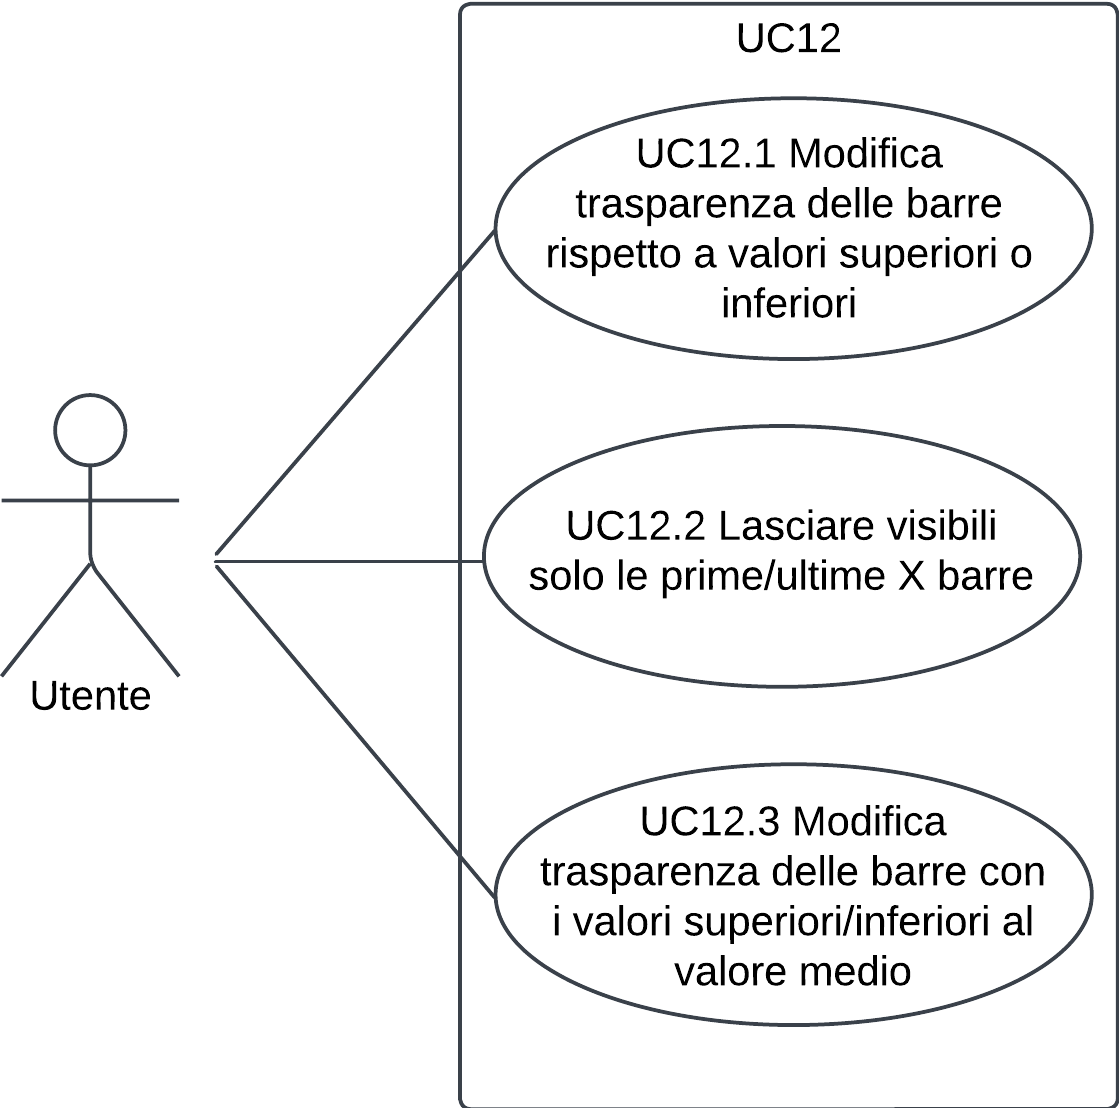
\includegraphics[scale=0.6]{template/images/UC12.png}
    \caption{\nameref*{UC:\arabic{UC}}}
\end{figure}
\UCdsc
{ % ATTORE
    \begin{itemize}
        \item Utente in ambiente 3D.
    \end{itemize}
}
{ % DESCRIZIONE
    \begin{itemize}
        \item Lo zoom consente all'utente di interagire con l'ambiente effettuando spostamenti lungo l'asse della profondità.
    \end{itemize}
}
{ % PRECONDIZIONI
    \begin{itemize}
        \item L'azione di zoom deve essere valida. Un'azione di zoom è valida se non va al di fuori un'area predefinita dal sistema;
        \item La telecamera si trova in una posizione arbitraria nello spazio.
    \end{itemize}
}
{ % POSTCONDIZIONI
    \begin{itemize}
        \item La telecamera si trova in una posizione diversa da quella iniziale in termini di profondità.
    \end{itemize}
}
{ % SCENARIO PRIMARIO
    \begin{itemize}
        \item L'utente interagisce con il sistema per compiere un'azione zoom.
    \end{itemize}
} 



\UseCase{Riposiziona telecamera alla posizione d’origine}
\begin{figure}[h!]\centering
    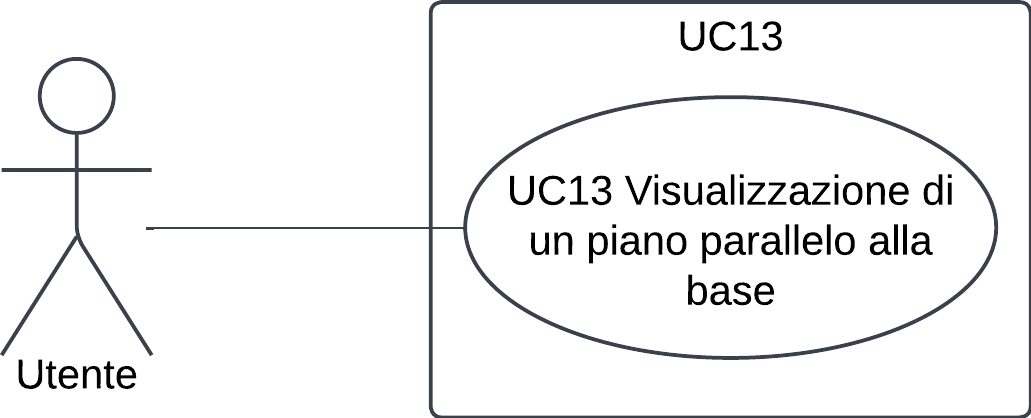
\includegraphics[scale=0.7]{template/images/UC13.png}
    \caption{\nameref*{UC:\arabic{UC}}}
\end{figure}
\UCdsc
{ % ATTORE
    \begin{itemize}
        \item Utente in ambiente 3D.
    \end{itemize}
}
{ % DESCRIZIONE
    \begin{itemize}
        \item Prevede il riposizionamento della telecamera al suo punto iniziale, la sua posizione alla creazione dell'ambiente 3D.
    \end{itemize}
}
{ % PRECONDIZIONI
    \begin{itemize}
        \item La telecamera si trova in una posizione arbitraria nello spazio.
    \end{itemize}
}
{ % POSTCONDIZIONI
    \begin{itemize}
        \item La telecamera si trova nella posizione predefinita iniziale.
    \end{itemize}
}
{ % SCENARIO PRIMARIO
    \begin{itemize}
        \item L'utente seleziona il comando per riposizionare la telecamera.
    \end{itemize}
} 



\UseCase{Vista di una barra in primo piano}
\begin{figure}[h!]\centering
    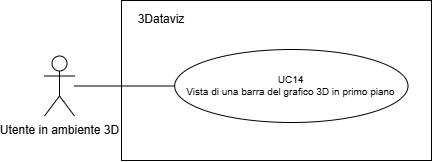
\includegraphics[scale=0.7]{template/images/UC14.png}
    \caption{\nameref*{UC:\arabic{UC}}}
\end{figure}
\UCdsc
{ % ATTORE
    \begin{itemize}
        \item Utente in ambiente 3D.
    \end{itemize}
}
{ % DESCRIZIONE
    \begin{itemize}
        \item La visualizzazione di una barra in primo piano consiste nel posizionare la telecamera in modo da massimizzare la visibilità di una specifica barra all'interno della scena, garantendo che sia sempre presente nel campo visivo dell'utente.
    \end{itemize}
}
{ % PRECONDIZIONI
    \begin{itemize}
        \item Il grafico è visibile;
        \item La telecamera si trova in una posizione arbitraria;
        \item L'utente ha selezionato un valore del dataset associato a una barra.
    \end{itemize}
}
{ % POSTCONDIZIONI
    \begin{itemize}
        \item La telecamera è stata riposizionata per mettere in primo piano la barra selezionata.
    \end{itemize}
}
{ % SCENARIO PRIMARIO
    \begin{itemize}
        \item L'utente seleziona un valore del dataset che corrisponde ad una barra sul grafico 3D.
    \end{itemize}
}


\UseCase{Visualizza dettagli di una barra del grafico 3D}
\begin{figure}[h!]\centering
    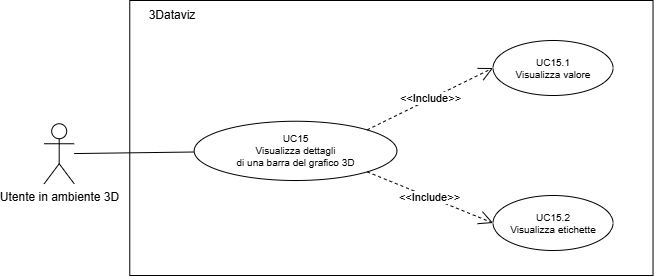
\includegraphics[scale=0.7]{template/images/UC15.png}
    \caption{\nameref*{UC:\arabic{UC}}}
\end{figure}
\UCdsc
{ % ATTORE
    \begin{itemize}
        \item Utente in ambiente 3D.
    \end{itemize}
}
{ % DESCRIZIONE
    \begin{itemize}
        \item L'utente può visualizzare i dettagli di una barra del grafico come il suo valore e le etichette a lei associate.
    \end{itemize}
}
{ % PRECONDIZIONI
    \begin{itemize}
        \item Il grafico è visibile;
        \item La barra è visibile.
    \end{itemize}
}
{ % POSTCONDIZIONI
    \begin{itemize}
        \item I dettagli della barra sono visibili.
    \end{itemize}
}
{ % SCENARIO PRIMARIO
    \begin{itemize}
        \item L'utente interagisce con la barra tramite hover o selezione.
    \end{itemize}
}

\SubUseCase{Visualizza valore}
\UCdsc
{ % ATTORE
    \begin{itemize}
        \item Utente in ambiente 3D.
    \end{itemize}
}
{ % DESCRIZIONE
    \begin{itemize}
        \item Visualizzazione del valore della barra.
    \end{itemize}
}
{ % PRECONDIZIONI
    \begin{itemize}
        \item I dettagli della barra sono visibili.
    \end{itemize}
}
{ % POSTCONDIZIONI
    \begin{itemize}
        \item Il valore della barra è visibile.
    \end{itemize}
}
{ % SCENARIO PRIMARIO
    \begin{itemize}
        \item Nessuna azione richiesta. 
    \end{itemize}
}

\SubUseCase{Visualizza etichette}
\UCdsc
{ % ATTORE
    \begin{itemize}
        \item Utente in ambiente 3D.
    \end{itemize}
}
{ % DESCRIZIONE
    \begin{itemize}
        \item Visualizzazione delle etichette associate alla barra.
    \end{itemize}
}
{ % PRECONDIZIONI
    \begin{itemize}
        \item I dettagli della barra sono visibili.
    \end{itemize}
}
{ % POSTCONDIZIONI
    \begin{itemize}
        \item Le etichette della barra sono visibili.
    \end{itemize}
}
{ % SCENARIO PRIMARIO
    \begin{itemize}
        \item Nessuna azione richiesta. 
    \end{itemize}
}

\UseCase{Filtra un numero N di valori}
\begin{figure}[h!]\centering
    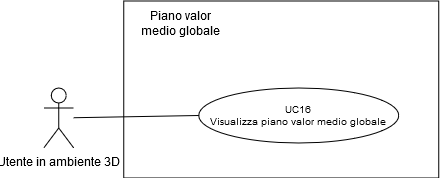
\includegraphics[scale=0.6]{template/images/UC16.png}
    \caption{\nameref*{UC:\arabic{UC}}}
\end{figure}
\UCdsc
{ % ATTORE
    \begin{itemize}
        \item Utente in ambiente 3D.
    \end{itemize}
}
{ % DESCRIZIONE
    \begin{itemize}
        \item Questo filtro consente all'utente di visualizzare solo le barre che corrispondono ai primi N valori più alti o più bassi. 
        N rappresenta il numero massimo di valori da considerare.
    \end{itemize}
}
{ % PRECONDIZIONI
    \begin{itemize}
        \item Il grafico è visibile;
    \end{itemize}
}
{ % POSTCONDIZIONI
    \begin{itemize}
        \item È stato applicato il filtro per visualizzare solo le prime N barre più alte o più basse.
    \end{itemize}
}
{ % SCENARIO PRIMARIO
    \begin{itemize}
        \item L'utente inserisce un numero N;
        \item L'utente seleziona il filtro;
        \item Il sistema aggiorna la visualizzazione del grafico, mostrando solo le barre che rientrano tra le prime N più alte o più basse.
    \end{itemize}
        % GENERALIZZAZIONI
        \item \textbf{Generalizzazioni:} \begin{itemize}
            \item UC16.1 - Filtra N valori più alti;
            \item UC16.2 - Filtra N valori più bassi.
        \end{itemize}
}

\SubUseCase{Filtra N valori più alti}
\UCdsc
{ % ATTORE
    \begin{itemize}
        \item Utente in ambiente 3D.
    \end{itemize}
}
{ % DESCRIZIONE
    \begin{itemize}
        \item L'utente decide di evidenziare i N valori più alti, rendendo visibili le barre corrispondenti.
    \end{itemize}
}
{ % PRECONDIZIONI
    \begin{itemize}
        \item Il grafico è visibile;
        \item L'utente ha scelto il filtro rispetto a numero N di valori.
    \end{itemize}
}
{ % POSTCONDIZIONI
    \begin{itemize}
        \item Le barre che non rientrano nelle prime N più alte diventano meno opache (più trasparenti).
    \end{itemize}
}
{ % SCENARIO PRIMARIO
    \begin{itemize}
        \item L'utente seleziona l'opzione per visualizzare le N barre più alte.
    \end{itemize}
}

\SubUseCase{Filtra N valori più bassi}
\UCdsc
{ % ATTORE
    \begin{itemize}
        \item Utente in ambiente 3D.
    \end{itemize}
}
{ % DESCRIZIONE
    \begin{itemize}
        \item L'utente decide di evidenziare i N valori più bassi, rendendo visibili le barre corrispondenti.
    \end{itemize}
}
{ % PRECONDIZIONI
    \begin{itemize}
        \item Il grafico è visibile;
        \item L'utente ha scelto il filtro su numero N di valori.
    \end{itemize}
}
{ % POSTCONDIZIONI
    \begin{itemize}
        \item Le barre che non rientrano nelle prime N più basse diventano meno opache (più trasparenti).
    \end{itemize}
}
{ % SCENARIO PRIMARIO
    \begin{itemize}
        \item L'utente seleziona l'opzione per visualizzare le N barre più basse.
    \end{itemize}
}

\UseCase{Filtra rispetto a un valore}
\begin{figure}[H]\centering
    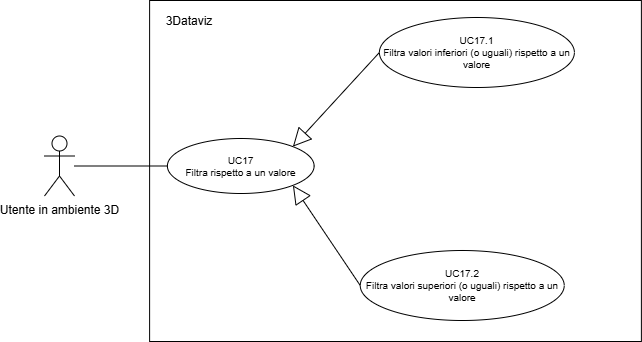
\includegraphics[scale=0.7]{template/images/UC17.png}
    \caption{\nameref*{UC:\arabic{UC}}}
\end{figure}
\UCdsc
{ % ATTORE
    \begin{itemize}
        \item Utente in ambiente 3D.
    \end{itemize}
}
{ % DESCRIZIONE
    \begin{itemize}
        \item Questo filtro consente all'utente di visualizzare solo le barre che hanno un valore superiore, inferiore o uguale rispetto a un valore scelto dall’utente. 
    \end{itemize}
}
{ % PRECONDIZIONI
    \begin{itemize}
        \item Il grafico è visibile.
    \end{itemize}
}
{ % POSTCONDIZIONI
    \begin{itemize}
        \item È stato applicato il filtro per visualizzare solo le barre con un valore superiore, inferiore o uguali;
        rispetto a un valore scelta dall’utente.
    \end{itemize}
}
{ % SCENARIO PRIMARIO
    \begin{itemize}
        \item L’utente seleziona un valore;
        \item Il sistema aggiorna la visualizzazione del grafico, evidenziando le barre che rientrano nella condizione scelta.
    \end{itemize}
  % GENERALIZZAZIONI
        \item \textbf{Generalizzazioni:} \begin{itemize}
            \item UC17.1 - Filtra valori inferiori (o uguali) rispetto a un valore;
            \item UC17.2 - Filtra valori superiori (o uguali) rispetto a un valore.
        \end{itemize}
    
}


\SubUseCase{Filtra valori inferiori (o uguali) rispetto a un valore}
\begin{figure}[H]\centering
    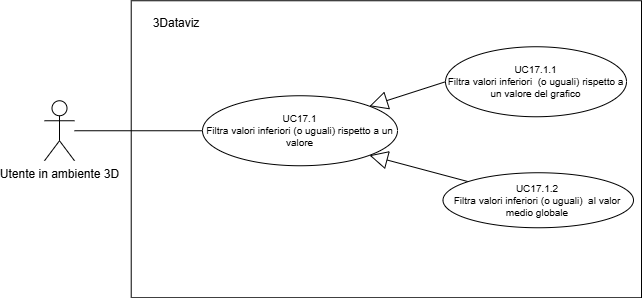
\includegraphics[scale=0.7]{template/images/UC17.1.png}
    \caption{\nameref*{UC:\arabic{UC}}}
\end{figure}
\UCdsc
{ % ATTORE
    \begin{itemize}
        \item Utente in ambiente 3D.
    \end{itemize}
}
{ % DESCRIZIONE
    \begin{itemize}
        \item L'utente decide di evidenziare i valori inferiori (o uguali) rispetto a un valore, rendendo visibili le barre corrispondenti a questo criterio.
    \end{itemize}
}
{ % PRECONDIZIONI
    \begin{itemize}
        \item Il grafico è visibile;
        \item L'utente ha scelto il filtro rispetto a un valore.
    \end{itemize}
}
{ % POSTCONDIZIONI
    \begin{itemize}
        \item Le barre con valori che non soddisfano il criterio di essere inferiori (o uguali) diventano meno opache(più trasparenti).
    \end{itemize}
}
{ % SCENARIO PRIMARIO
    \begin{itemize}
        \item L'utente seleziona l'opzione per visualizzare le barre inferiori (o uguali).
    \end{itemize}
    % GENERALIZZAZIONI
    \item \textbf{Generalizzazioni:} \begin{itemize}
        \item UC17.1.1 - Filtra valori inferiori (o uguali) rispetto a un valore del grafico;
        \item UC17.2.2 - Filtra valori inferiori (o uguali) rispetto al valor medio globale.
    \end{itemize}
}



\SubSubUseCase{Filtra valori inferiori (o uguali) rispetto a un valore del grafico}
\UCdsc
{ % ATTORE
    \begin{itemize}
        \item Utente in ambiente 3D.
    \end{itemize}
}
{ % DESCRIZIONE
    \begin{itemize}
        \item L'utente decide di evidenziare i valori inferiori (o uguali) rispetto a un valore del grafico, rendendo visibili le barre corrispondenti a questo criterio.
    \end{itemize}
}
{ % PRECONDIZIONI
    \begin{itemize}
        \item Il grafico è visibile;
        \item L'utente ha scelto il filtro di valori inferiori (o uguali).
    \end{itemize}
}
{ % POSTCONDIZIONI
    \begin{itemize}
        \item Le barre con valori che non soddisfano il criterio di essere inferiori (o uguali) rispetto a un valore del grafico selezionato diventano meno opache(più trasparenti).
    \end{itemize}
}
{ % SCENARIO PRIMARIO
    \begin{itemize}
        \item L'utente seleziona l'opzione per visualizzare le barre inferiori (o uguali) rispetto a un valore del grafico.
    \end{itemize}
}


\SubSubUseCase{Filtra valori inferiori (o uguali) rispetto al valor medio globale}
\UCdsc
{ % ATTORE
    \begin{itemize}
        \item Utente in ambiente 3D.
    \end{itemize}
}
{ % DESCRIZIONE
    \begin{itemize}
        \item L'utente decide di evidenziare i valori inferiori (o uguali) rispetto al valor medio globale, rendendo visibili le barre corrispondenti a questo criterio.
    \end{itemize}
}
{ % PRECONDIZIONI
    \begin{itemize}
        \item Il grafico è visibile;
        \item L'utente ha scelto il filtro di valori inferiori (o uguali).
    \end{itemize}
}
{ % POSTCONDIZIONI
    \begin{itemize}
        \item Le barre con valori che non soddisfano il criterio di essere inferiori (o uguali) rispetto al valor medio globale diventano meno opache(più trasparenti).
    \end{itemize}
}
{ % SCENARIO PRIMARIO
    \begin{itemize}
        \item L'utente seleziona l'opzione per visualizzare le barre inferiori (o uguali) rispetto al valor medio globale.
    \end{itemize}
}




\SubUseCase{Filtra valori superiori (o uguali) rispetto a un valore}
\begin{figure}[H]\centering
    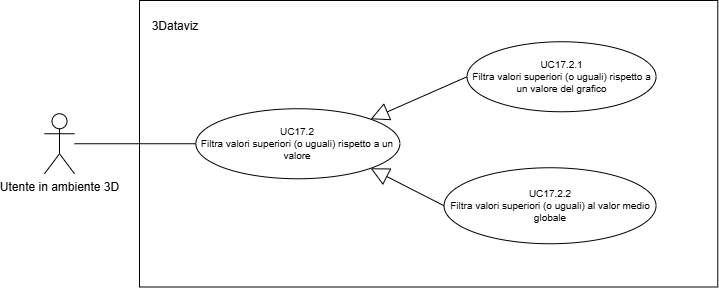
\includegraphics[scale=0.6]{template/images/UC17.2.png}
    \caption{\nameref*{UC:\arabic{UC}}}
\end{figure}
\UCdsc
{ % ATTORE
    \begin{itemize}
        \item Utente in ambiente 3D.
    \end{itemize}
}
{ % DESCRIZIONE
    \begin{itemize}
        \item L'utente decide di evidenziare i valori superiori (o uguali) rispetto a un valore, rendendo visibili le barre corrispondenti a questo criterio.
    \end{itemize}
}
{ % PRECONDIZIONI
    \begin{itemize}
        \item Il grafico è visibile;
        \item L'utente ha scelto il filtro rispetto a un valore.
    \end{itemize}
}
{ % POSTCONDIZIONI
    \begin{itemize}
        \item Le barre dei valori che non rientrano in questa condizione diventano meno opache(più trasparenti).
    \end{itemize}
}
{ % SCENARIO PRIMARIO
    \begin{itemize}
        \item L'utente seleziona l'opzione per visualizzare le barre superiori (o uguali).
    \end{itemize}
    % GENERALIZZAZIONI
    \item \textbf{Generalizzazioni:} \begin{itemize}
        \item UC17.1.1 - Filtra valori superiori (o uguali) rispetto a un valore del grafico;
        \item UC17.2.2 - Filtra valori superiori (o uguali) rispetto al valor medio globale.
    \end{itemize}
}


\SubSubUseCase{Filtra valori superiori (o uguali) rispetto a un valore del grafico}
\UCdsc
{ % ATTORE
    \begin{itemize}
        \item Utente in ambiente 3D.
    \end{itemize}
}
{ % DESCRIZIONE
    \begin{itemize}
        \item L'utente decide di evidenziare i valori superiori (o uguali) rispetto a un valore del grafico, rendendo visibili le barre corrispondenti a questo criterio.
    \end{itemize}
}
{ % PRECONDIZIONI
    \begin{itemize}
        \item Il grafico è visibile;
        \item L'utente ha scelto il filtro di valori superiori (o uguali).
    \end{itemize}
}
{ % POSTCONDIZIONI
    \begin{itemize}
        \item Le barre con valori che non soddisfano il criterio di essere superiori (o uguali) rispetto a un valore del grafico selezionato diventano meno opache(più trasparenti).
    \end{itemize}
}
{ % SCENARIO PRIMARIO
    \begin{itemize}
        \item L'utente seleziona l'opzione per visualizzare le barre superiori (o uguali) rispetto a un valore del grafico.
    \end{itemize}
}


\SubSubUseCase{Filtra valori superiori (o uguali) rispetto al valor medio globale}
\UCdsc
{ % ATTORE
    \begin{itemize}
        \item Utente in ambiente 3D.
    \end{itemize}
}
{ % DESCRIZIONE
    \begin{itemize}
        \item L'utente decide di evidenziare i valori superiori (o uguali) rispetto al valor medio globale, rendendo visibili le barre corrispondenti a questo criterio.
    \end{itemize}
}
{ % PRECONDIZIONI
    \begin{itemize}
        \item Il grafico è visibile;
        \item L'utente ha scelto il filtro di valori superiori (o uguali).
    \end{itemize}
}
{ % POSTCONDIZIONI
    \begin{itemize}
        \item Le barre con valori che non soddisfano il criterio di essere superiori (o uguali) rispetto al valor medio globale diventano meno opache(più trasparenti).
    \end{itemize}
}
{ % SCENARIO PRIMARIO
    \begin{itemize}
        \item L'utente seleziona l'opzione per visualizzare le barre superiori (o uguali) rispetto al valor medio globale.
    \end{itemize}
}




\UseCase{Inserimento di un valore}
\UCdsc
{ % ATTORE
    \begin{itemize}
        \item Utente in ambiente 3D.
    \end{itemize}
}
{ % DESCRIZIONE
    \begin{itemize}
        \item Questo caso d'uso consente all'utente di inserire un valore numerico positivo che sarà utilizzato per applicare un filtro sui dati visualizzati nel grafico 3D. L'utente può inserire un valore per determinare il numero di barre da visualizzare, ad esempio per filtrare i N valori più alti o più bassi del grafico, in base al tipo di filtro selezionato.
    \end{itemize}
}
{ % PRECONDIZIONI
    \begin{itemize}
        \item Il grafico è visibile;
        \item L'utente ha selezionato il filtraggio di un numero N di valori.
    \end{itemize}
}
{ % POSTCONDIZIONI
    \begin{itemize}
        \item Il valore desiderato è stato inserito nel campo corrispondente.
    \end{itemize}
}
{ % SCENARIO PRIMARIO
    \begin{itemize}
        \item L'utente inserisce un valore valido nel campo corrispondente.
    \end{itemize}
}



\UseCase{Visualizza piano del valor medio}
\begin{figure}[h!]\centering
    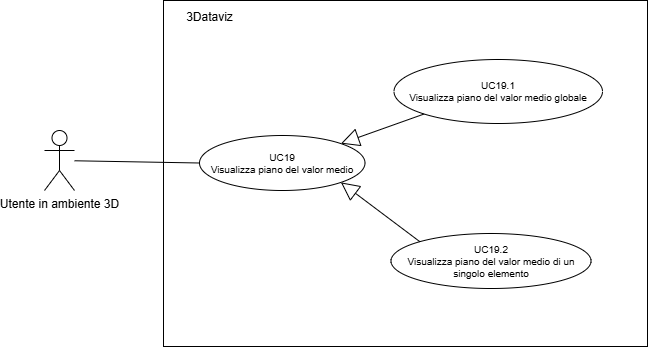
\includegraphics[scale=0.7]{template/images/UC19.png}
    \caption{\nameref*{UC:\arabic{UC}}}
\end{figure}
\UCdsc
{ % ATTORE
    \begin{itemize}
        \item Utente in ambiente 3D.
    \end{itemize}
}
{ % DESCRIZIONE
    \begin{itemize}
        \item Generazione di un piano parallelo alla base inserito nel grafico 3D per evidenziare un valor medio.
    \end{itemize}
}
{ % PRECONDIZIONI
    \begin{itemize}
        \item Il grafico è visibile.
    \end{itemize}
}
{ % POSTCONDIZIONI
    \begin{itemize}
        \item Il piano che rappresenta il valor medio è visibile.
    \end{itemize}
}
{ % SCENARIO PRIMARIO
    \begin{itemize}
        \item L'utente seleziona l'opzione per visualizzare il valor medio.
    \end{itemize}
}


\SubUseCase{Visualizza piano del valor medio globale}
\UCdsc
{ % ATTORE
    \begin{itemize}
        \item Utente in ambiente 3D.
    \end{itemize}
}
{ % DESCRIZIONE
    \begin{itemize}
        \item Un piano, parallelo alla base, viene inserito nel grafico 3D per evidenziare il valor medio globale dei dati.
    \end{itemize}
}
{ % PRECONDIZIONI
    \begin{itemize}
        \item Il grafico è visibile.
    \end{itemize}
}
{ % POSTCONDIZIONI
    \begin{itemize}
        \item Il piano che rappresenta il valor medio globale è visibile.
    \end{itemize}
}
{ % SCENARIO PRIMARIO
    \begin{itemize}
        \item L'utente seleziona l'opzione per visualizzare il valor medio;
        \item L'utente seleziona l'opzione del valor medio globale.
    \end{itemize}
}

\SubUseCase{Visualizza piano valor medio di un singolo elemento}
\UCdsc
{ % ATTORE
    \begin{itemize}
        \item Utente in ambiente 3D.
    \end{itemize}
}
{ % DESCRIZIONE
    \begin{itemize}
        \item Un piano, parallelo alla base, viene inserito nel grafico 3D per evidenziare il valor medio di un singolo elemento tra quelli nel dataset, cioè il valor medio rispetto a un unico asse di etichetta.
    \end{itemize}
}
{ % PRECONDIZIONI
    \begin{itemize}
        \item Il grafico è visibile.
    \end{itemize}
}
{ % POSTCONDIZIONI
    \begin{itemize}
        \item Il piano che rappresenta il valor medio di un singolo elemento è visibile.
    \end{itemize}
}
{ % SCENARIO PRIMARIO
    \begin{itemize}
        \item L'utente seleziona l'opzione per visualizzare il valor medio;
        \item L'utente seleziona l'etichetta su quale genererare il valor medio.
    \end{itemize}
}

